\section{Proximity-Based Approaches}


\begin{frame}
  \frametitle{Proximity-Based Approaches: \\
    Distance-Based vs. Density-Based Outlier Detection}
  \begin{itemize}
  \item \textbf{Intuition:}
    \begin{itemize}
    \item Objects that are \textbf{far away from the others} are outliers.
    \end{itemize}
  \item \textbf{Assumption of proximity-based approach:}
    \begin{itemize}
    \item The proximity of an outlier deviates significantly from that of most of the others in the data set.
    \end{itemize}
  \item \textbf{Two types of proximity-based outlier-detection methods:}
    \begin{itemize}
    \item \textbf{\color{airforceblue}Distance-based} outlier detection:
      \begin{itemize}
      \item An object $\mathbf{o}$ is an outlier, \\
        if its neighborhood does not have enough other points.
      \end{itemize}
    \item \textbf{\color{airforceblue}Density-based} outlier detection:
      \begin{itemize}
      \item An object $\mathbf{o}$ is an outlier, \\
        if its density is relatively much lower than that of its neighbors.
      \end{itemize}
    \end{itemize}
  \end{itemize}
\end{frame}


\begin{frame}
  \frametitle{Distance-Based Outlier Detection }
  \begin{itemize}
  \item For each object $\mathbf{o}$, examine the number of other objects \\
    in the \textbf{r-neighborhood} of $\mathbf{o}$, \\
    where $r$ is a user-specified \textbf{distance threshold}.
  \item An object $\mathbf{o}$ is an outlier if most (taking $\pi$ as a \textbf{fraction threshold}) \\
    of the objects in $\mathbf{D}$ are far away from $\mathbf{o}$, i.e., not in the $r$-neighborhood of $\mathbf{o}$.
  \end{itemize}
  \begin{itemize}
  \item \textbf{An object $\mathbf{o}$ is a $\mathbf{DB}(r, \pi)$ outlier, iff}
    \begin{align}
      \frac{||\{\mathbf{o'} \; \vert \; d(\mathbf{o},\mathbf{o'}) \leq r \}|| }{||D||} \leq \pi.
    \end{align}
  \item Equivalently, one can check the distance between $\mathbf{o}$ and its \\
    $k$-th nearest neighbor $\mathbf{o}_k$, where $k=\lceil \pi ||D||\rceil$                       . \\
  \item $\mathbf{o}$ is an outlier, if $d(\mathbf{o}, \mathbf{o}_k) > r$.
  \end{itemize}
\end{frame}


\begin{frame}
  \frametitle{Distance-Based Outlier Detection (2)}
  \begin{itemize}
  \item \textbf{Efficient computation: {\color{airforceblue}Nested-loop algorithm}:}
    \begin{itemize}
    \item For any object $\mathbf{o}_i$, calculate its distance from other objects, \\
      and count the number of other objects in the $r$-neighborhood.
    \item If $\pi \cdot n$ other objects are within $r$-distance, terminate the inner loop.
    \item Otherwise, $\mathbf{o}_i$ is a $\mathbf{DB}(r, \pi)$ outlier.
    \end{itemize}
  \item \textbf{Efficiency:}
    \begin{itemize}
    \item Actually, CPU time is not $\mathcal{O}(n^2)$ but linear to the data set size,\\
      since for most non-outlier objects, the inner loop terminates early.
    \end{itemize}
  \end{itemize}
\end{frame}


\begin{frame}
  \frametitle{Distance-Based Outlier Detection (3)}
  \begin{itemize}
  \item \textbf{Why is efficiency still a concern?}
    \begin{itemize}
    \item If the complete set of objects cannot be held in main memory, \\
      there is significant cost for I/O swapping.
    \end{itemize}
  \item \textbf{The major cost:}
    \begin{itemize}
    \item[1.] Each object is tested against the whole data set, \\
      why not only against its close neighbors?
    \item[2.] Objects are checked one by one, why not group by group?
    \end{itemize}
  \end{itemize}
\end{frame}


\begin{frame}
  \frametitle{Distance-Based Outlier Detection:A Grid-Based Method}
  \begin{itemize}
  \item \textbf{CELL:}
    \begin{itemize}
    \item Data space is partitioned into a multi-D grid.
    \item Each cell is a hyper cube with diagonal length $\frac{r}{2}$.
      \begin{itemize}
      \item $r$-distance threshold parameter.
      \item $l$-dimensions: edge of each cell $r / (2\sqrt{l})$ long.
      \end{itemize}
    \end{itemize}
  \item \textbf{Level-1 cells:}
    \begin{itemize}
    \item Immediately next to cell $\mathbf{C}$.
    \item For any possible point $\mathbf{x}$ in $\mathbf{C}$ and \\
      any possible point $\mathbf{y}$ in a level-1 cell: $d(x,y) \leq r$.
    \end{itemize}
  \item \textbf{Level-2 cells:}
    \begin{itemize}
    \item One or two cells away from $\mathbf{C}$.
    \item For any possible point $\mathbf{x}$ in cell $\mathbf{C}$ and \\
      any point $\mathbf{y}$ such that $d(x,y) \geq r$, $\mathbf{y}$ is in a level-2 cell.
    \item
    \end{itemize}
  \end{itemize}
  \tikzoverlay at (10cm,6cm) {\includegraphics[width=0.25\textwidth]{img/grid8.png}};
\end{frame}


\begin{frame}
  \frametitle{Distance-Based Outlier Detection: A Grid-Based Method (2)}
  \begin{itemize}
  \item Total number of objects in cell $\mathbf{C}$: $a$.
  \item Total number of objects in level-1 cells: $b_1$.
  \item Total number of objects in level-2 cells: $b_2$.
  \end{itemize}
  \begin{itemize}
  \item \textbf{Level-1 cell pruning rule}:
    \begin{itemize}
    \item If $a + b_1 > \lceil \pi n \rceil$, then every object $\mathbf{o}$ in $\mathbf{C}$ is not a $\mathbf{DB}(r, \pi)$ outlier, because all objects in $\mathbf{C}$ and the level-1 cells are in the $r$-neighborhood of $\mathbf{o}$,and there are at least $\lceil \pi n \rceil$ such objects.
    \end{itemize}
  \item \textbf{Level-2 cell pruning rule:}
    \begin{itemize}
    \item If $a + b_1 + b_2 < \lceil \pi n \rceil + 1$, then all objects in $\mathbf{C}$ are $\mathbf{DB}(r, \pi)$ outliers, because all of their $r$-neighborhoods have less than $\lceil \pi n \rceil$ other objects.
    \end{itemize}
  \item \textbf{Only need to check the objects that cannot be pruned.}
    \begin{itemize}
    \item Even for such an object $\mathbf{o}$, \\
      only need to compute the distance between $\mathbf{o}$ and the objects in level-2 cells.
      \begin{itemize}
      \item Since beyond level-2, distance from $\mathbf{o}$ is more than $r$.
      \end{itemize}
    \end{itemize}
  \end{itemize}
\end{frame}


\begin{frame}
  \frametitle{Density-Based Outlier Detection}
  \begin{itemize}
  \item \textbf{\color{airforceblue}Local outliers:}
    \begin{itemize}
    \item Outliers compared to their local neighborhoods, not to global data distribution.
      \begin{itemize}
      \item In the figure, O1 and O2 are local outliers to C1, O3 is a global outlier, \\
        but O4 is not an outlier.
      \item However, distance of O1 and O2 to objects in dense cluster C1 \\
        is smaller than average distance in sparse cluster C2.
      \item Hence, O1 and O2 are not distance-based outliers.
      \end{itemize}
    \end{itemize}
  \item \textbf{\color{airforceblue}Intuition:}
    \begin{itemize}
    \item Density around \textbf{outlier} object \textbf{significantly different} \\
      from density around its neighbors.
    \end{itemize}
  \end{itemize}
  \tikzoverlay at (9.5cm,2cm) {
    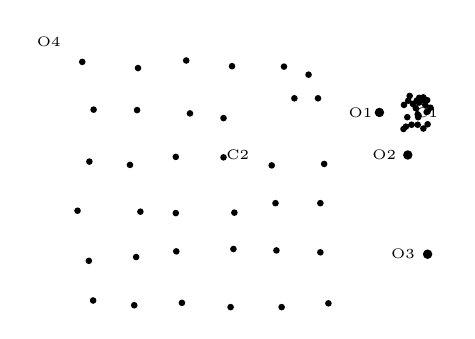
\begin{tikzpicture}[thick,scale=0.6, every node/.style={scale=5}]
      \fill (0.14, 0.02)  circle (0.7mm) (0.05, 0.86)  circle (0.7mm) (-0.19, 1.92)  circle (0.7mm) (0.06, 2.96)  circle (0.7mm) (0.15, 4.06)  circle (0.7mm) (-0.09, 5.07)  circle (0.7mm) (1.01, -0.08)  circle (0.7mm) (1.05, 0.94)  circle (0.7mm) (1.14, 1.9)  circle (0.7mm) (0.92, 2.89)  circle (0.7mm) (1.07, 4.05)  circle (0.7mm) (1.09, 4.94)  circle (0.7mm) (2.02, -0.03)  circle (0.7mm) (1.9, 1.06)  circle (0.7mm) (1.89, 1.87)  circle (0.7mm) (1.89, 3.06)  circle (0.7mm) (2.19, 3.98)  circle (0.7mm) (2.11, 5.1)  circle (0.7mm) (3.05, -0.12)  circle (0.7mm) (3.11, 1.11)  circle (0.7mm) (3.13, 1.88)  circle (0.7mm) (2.9, 3.05)  circle (0.7mm) (2.9, 3.88)  circle (0.7mm) (3.08, 4.98)  circle (0.7mm) (4.13, -0.12)  circle (0.7mm) (4.02, 1.08)  circle (0.7mm) (4.0, 2.08)  circle (0.7mm) (3.92, 2.88)  circle (0.7mm) (4.4, 4.3)  circle (0.7mm) (4.18, 4.97)  circle (0.7mm) (5.12, -0.04)  circle (0.7mm) (4.95, 1.04)  circle (0.7mm) (4.95, 2.08)  circle (0.7mm) (5.03, 2.91)  circle (0.7mm) (4.9, 4.3)  circle (0.7mm) (4.7, 4.8)  circle (0.7mm);

      % cluster
      \fill (7.22, 4.02)  circle (0.7mm) (7.01, 3.74)  circle (0.7mm) (7.17, 4.16)  circle (0.7mm) (7.04, 4.31)  circle (0.7mm) (7.28, 4.1)  circle (0.7mm) (7.22, 3.75)  circle (0.7mm) (6.99, 4.25)  circle (0.7mm) (7.13, 3.66)  circle (0.7mm) (7.03, 3.93)  circle (0.7mm) (6.84, 4.35)  circle (0.7mm) (6.72, 4.16)  circle (0.7mm) (7.14, 4.27)  circle (0.7mm) (6.88, 3.74)  circle (0.7mm) (7.04, 4.21)  circle (0.7mm) (6.79, 3.9)  circle (0.7mm) (7.01, 3.96)  circle (0.7mm) (7.13, 4.32)  circle (0.7mm) (6.71, 3.65)  circle (0.7mm) (6.76, 3.7)  circle (0.7mm) (7.21, 4.26)  circle (0.7mm) (7.02, 3.9)  circle (0.7mm) (7.2, 4.01)  circle (0.7mm) (6.91, 4.18)  circle (0.7mm) (6.81, 4.25)  circle (0.7mm) (6.97, 4.09)  circle (0.7mm);

      % outlier O3
      \fill (7.22, 1)  circle (1mm);
      \node[scale = 0.2] at (6.7, 1) {\tiny O3};

      % O1
      \fill (6.2, 4)  circle (1mm);
      \node[scale = 0.2] at (5.8, 4) {\tiny O1};

      % O2
      \fill (6.8, 3.1)  circle (1mm);
      \node[scale = 0.2] at (6.3, 3.1) {\tiny O2};
      \node[scale = 0.2] at (7.2, 4) {\tiny C1};
      \node[scale = 0.2] at (3.2, 3.1) {\tiny C2};
      \node[scale = 0.2] at (-0.8, 5.5) {\tiny O4};
    \end{tikzpicture}};
\end{frame}


\begin{frame}
  \frametitle{Density-Based Outlier Detection (2)}
  \begin{itemize}
  \item \textbf{Method:}
    \begin{itemize}
    \item Use the \textbf{relative density} of an object against its neighbors \\
      as the indicator of the degree of the object being outliers
    \end{itemize}
  \item \textbf{{\color{airforceblue}$k$-distance} of an object $\mathbf{o}$:} $d_k(\mathbf{o})$.
  \item Distance $d(\mathbf{o}, \mathbf{p})$ between $\mathbf{o}$ and its $k$-nearest neighbour $p$.
    \begin{itemize}
    \item Test at least $k$ objects $\textbf{o'} \in \mathbf{D} - \{\mathbf{o}\}$ \\
      such that $d(\mathbf{o}, \mathbf{o'}) \leq d(\mathbf{o}, \mathbf{p})$.
    \item at most $k-1$ objects $\mathbf{o''} \in \mathbf{D} - \{\mathbf{o}\}$ \\
      such that $d(\mathbf{o}, \mathbf{o'}) > d(\mathbf{o}, \mathbf{p})$.
    \end{itemize}
  \item $k$-distance neighborhood of $\mathbf{o}$:
    \begin{itemize}
    \item $N_k(\mathbf{o}) = {\mathbf{o'} \; \vert \; \mathbf{o'} \in \mathbf{D}, d(\mathbf{o}, \mathbf{o'}) \leq d_k(\mathbf{o})}$.
    \item $N_k(\mathbf{o})$ could be bigger than $k$ \\
      since multiple objects may have identical distance to $\mathbf{o}$.
    \end{itemize}
  \end{itemize}
\end{frame}


\begin{frame}
  \frametitle{Local Outlier Factor}
  \begin{itemize}
  \item \textbf{\color{airforceblue}Reachability distance from $\mathbf{o'}$ to $\mathbf{o}$:}
    \begin{align*}
      \text{reachdist}_k(\mathbf{o'} \leftarrow \mathbf{o}) = \max \{d_k(\mathbf{o}), d(\mathbf{o},\mathbf{o'})\},
    \end{align*}
    \begin{itemize}
    \item where $k$ is a user-specified parameter.
    \end{itemize}
  \item \textbf{Local reachability density of $\mathbf{o}$:}
    \begin{align*}
      \resizebox{5cm}{!}{%
      $\text{ldr}_k(\mathbf{o}) = \frac{||N_k(\mathbf{o})||}{\sum_{\mathbf{o'} \in N_k(\mathbf{o})} \text{reachdist}_k(\mathbf{o'} \leftarrow \mathbf{o})}.$}
    \end{align*}
  \item \textbf{LOF (Local Outlier Factor) of $\mathbf{o}$:}
    \begin{itemize}
    \item The average of the ratio of local reachability of $\mathbf{o}$ and \\
      those of $\mathbf{o}$'s $k$-nearest neighbors.
      \begin{align*}
        \resizebox{8cm}{!}{%
        $\text{LOF}_k(\mathbf{o}) = \frac{\sum_{\mathbf{o'} \in N_k(\mathbf{o})} \frac{\text{lrd}_k(\mathbf{o'})}{\text{lrd}_k(\mathbf{o})}}{||N_k(\mathbf{o})||} =
        \sum_{\mathbf{o'} \in N_k(\mathbf{o})} \text{lrd}_k(\mathbf{o'}) \cdot \sum_{\mathbf{o'} \in N_k(\mathbf{o})} \text{reachdist}_k(\mathbf{o'} \leftarrow \mathbf{o}).$}
      \end{align*}
    \item The lower the local reachability density of $\mathbf{o}$, and the higher the local reachability density of the $k$-NN of $\mathbf{o}$, the higher LOF.
    \item This captures a local outlier whose local density is relatively low comparing to the local densities of its $k$-NN.
    \end{itemize}
  \end{itemize}
  \tikzoverlay at (11cm,6.5cm){\includegraphics[width=0.25\textwidth]{img/density.png}};
\end{frame}
